\documentclass[a4paper,english,abstract=on]{scrartcl}

\usepackage{mathtools} % loads amsmath and fixes its bugs in Unicode & XeLaTeX/LuaLaTeX 
\usepackage[english]{babel}
\usepackage[]{unicode-math} % provides Unicode Math support for XeLaTeX/LuaLaTeX 
\usepackage{xcolor}
\usepackage{graphicx}
\usepackage[pdfborder={0 0 0}]{hyperref}
\usepackage[autostyle=true]{csquotes}
\usepackage[backend=biber, style=numeric-comp]{biblatex}

\usepackage{fontspec}
\newfontfamily{\ttconsolas}{Consolas}
\usepackage{listings}
\setmonofont{Consolas}
\lstset{
	breaklines=true,
	tabsize=2,
	basicstyle=\ttfamily\small,
}

\addbibresource{literatur.bib}

\title{Exercise 5 Report}
\subtitle{Gruppe 16}
\author{Anastasiia Rubanovych\and Sebastian Funck}
\date{\today}

\begin{document}

\maketitle

\subsection*{1)}
\textbf{INSERT}
\begin{lstlisting}{Name}
> db.films.insert({ 
	title: "Iron Man 3", 
	year: 2013, 
	genre: [ "Action", "Adventure", "Sci-Fi", ], 
	actors: [ "Downey Jr., Robert", "Paltrow, Gwyneth",]
})
WriteResult({ "nInserted" : 1 })
\end{lstlisting}
~\\
\textbf{QUERY}
\begin{lstlisting}{Name}
> db.films.find(
	{ year: {$gt: 2009,$lte: 2011}, title: /^T/},
	{ _id: 0,title: 1}
)
WriteResult({ "nInserted" : 1 })
\end{lstlisting}
~\\
\textbf{UPDATE}
\begin{lstlisting}{Name}
> db.films.update(
	{title: "Star Trek Into Darkness"},
	{$set: {rating: 6.4}}
)
WriteResult({"nMatched": 1, "nUpserted":0, "nModified":1 })
\end{lstlisting}
~\\
\textbf{DELETE}
\begin{lstlisting}{Name}
> db.films.remove({title: /^T/})
WriteResult({ "nRemoved" : 2 })
\end{lstlisting}

\newpage
\textbf{INDEXING}
\begin{lstlisting}{Name}
> db.movies.find({rating: {$gt: 6.14,$lt: 7.78}})
           .explain("executionStats")
{
...
"executionTimeMillis" : 172,
...
}

> db.movies.ensureIndex({rating: 1})
> db.movies.find({rating: {$gt: 6.14,$lt: 7.78}})
           .explain("executionStats")
{
...
"executionTimeMillis" : 118,
...
}
\end{lstlisting}
\subsection*{2)}
We implemented following functionality:
\begin{itemize}
	\item {\ttconsolas findMovieByTitle}\\
	We used {\ttconsolas movies.find(new Document("title", title)).first()} for this method because we couldn't find an equivalent to {\ttconsolas findOne}.
	\item {\ttconsolas getBestMovies}\\
	We combined {\ttconsolas Filters.and} and {\ttconsolas Filters.gt} to filter for movies that have a rating and number of votes larger than the given arguments.
	\item {\ttconsolas getByGenre}\\
	We used {\ttconsolas Filters.all} to filter for all movies that have the given filters. We also added a {\ttconsolas .replace(" ","")} so the user can have whitespaces in the query.
	\item {\ttconsolas searchByPrefix}\\
	We applied a {\ttconsolas Filters.regex} with pattern {\ttconsolas $\wedge$}\textit{prefix} to filter for movies beginning with the given prefix.
	\item {\ttconsolas getTweetedMovies}\\
	To find movies that have been tweeted about we comined a {\ttconsolas Filters.exists("tweets")} and a {\ttconsolas Filters.ne("tweets", null)} filter. In theory the {\ttconsolas Filters.nin} filter is redundant as movies without tweets don't have the tweets-field, but added the null-check for robustness.
	\item {\ttconsolas saveMovieComment}\\
	Executes a {\ttconsolas updateOne} for a given movie Object-ID and sets the new comment.
	\item {\ttconsolas getByTweetsKeywordRegex}\\
	For this method we used a 2 phase query. First we find tweets that match the keyword-regex and collect the distinct values of the {\ttconsolas movies} field. Afterwards we fetch the movies by the values we collected in the first step.
	\item {\ttconsolas searchTweets}\\
	After the index has been created on {\ttconsolas text} and {\ttconsolas user.name} we use {\ttconsolas Filters.text} to do a full-text search over the indexed fields.
	\item {\ttconsolas getNewestTweets}\\
	We fetch the latest object-ids to find the correspoding tweets.
	\item {\ttconsolas getGeotaggedTweets}\\
	We search for tweets that have the field {\ttconsolas "coordinates"} and it's not null.
	\item {\ttconsolas saveFile}
	We use {\ttconsolas GridFSBucket.uploadFromStream} to upload the file.
	\item {\ttconsolas getFile}
	First we try to fetch the first GridFSFile that matches the given filename via {\ttconsolas GridFSBucket.find}. If that file doesn't exists we fetch the backup file {\ttconsolas sample.png} from that we know it is available.
\end{itemize}
\textbf{findMovieByTitle / getFile / saveFile / saveMovieComment}\\
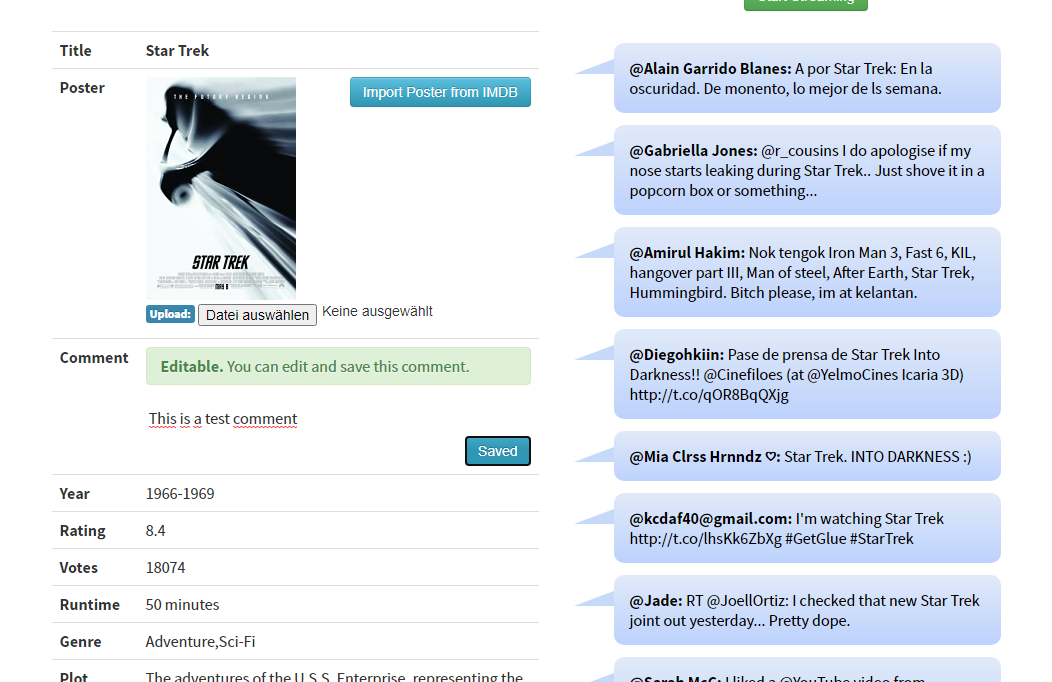
\includegraphics[width=\textwidth,height=\textheight,keepaspectratio]{startrek.png}\\
\newpage
\textbf{getByGenre}\\
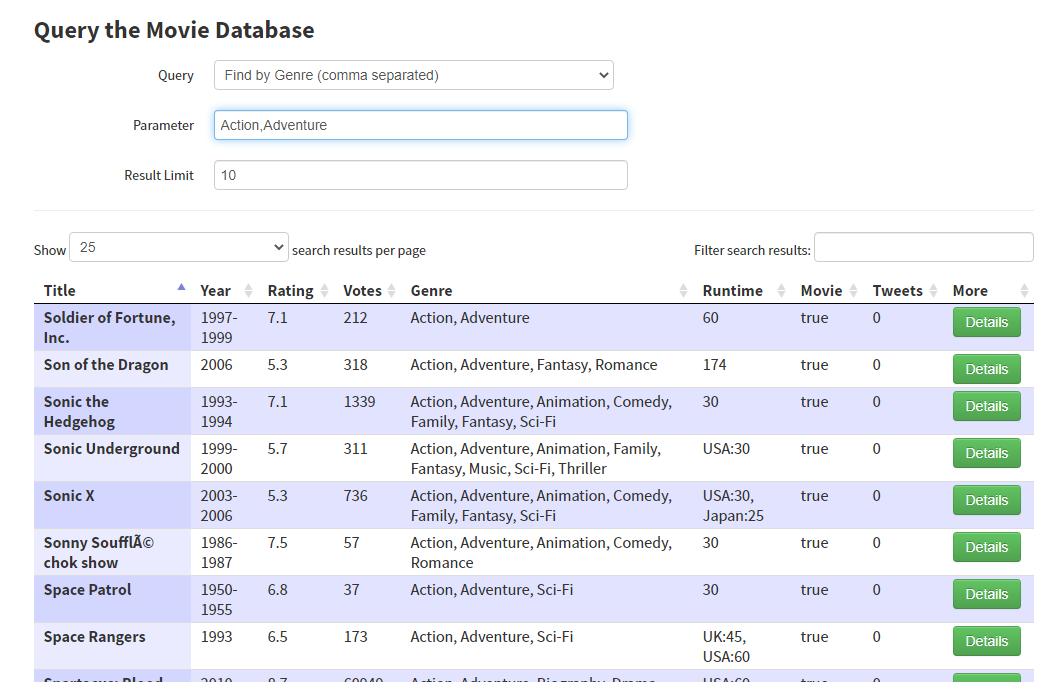
\includegraphics[width=\textwidth,height=\textheight,keepaspectratio]{search_genre_list.png}\\
\textbf{searchTweets}\\
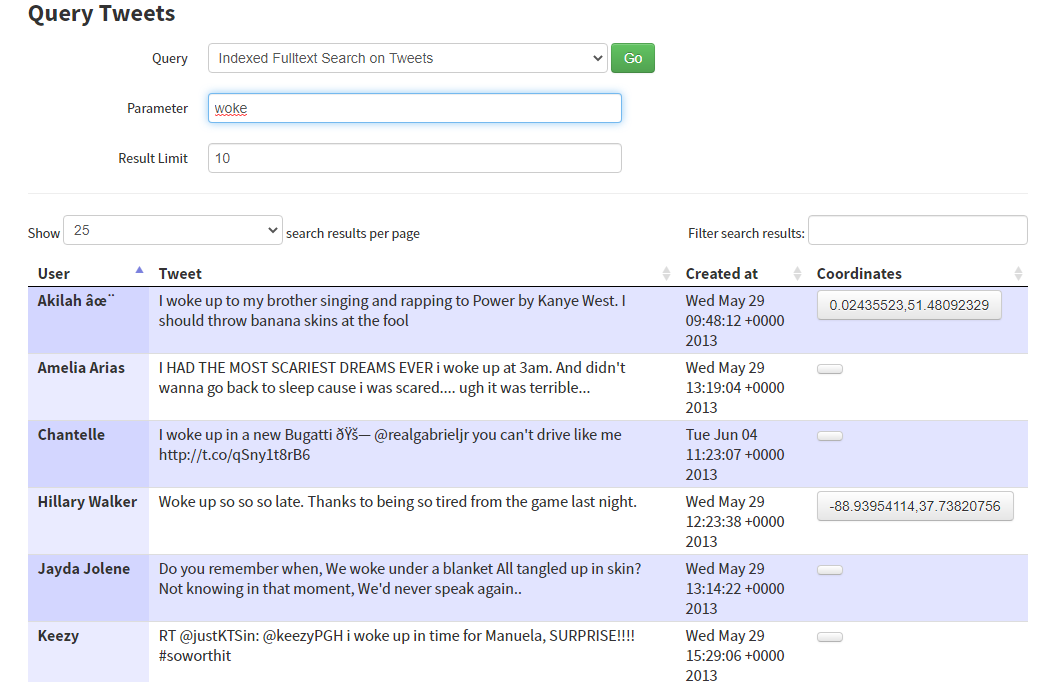
\includegraphics[width=\textwidth,height=\textheight,keepaspectratio]{search_full_text.png}\\
\newpage
\textbf{getNewestTweets}\\
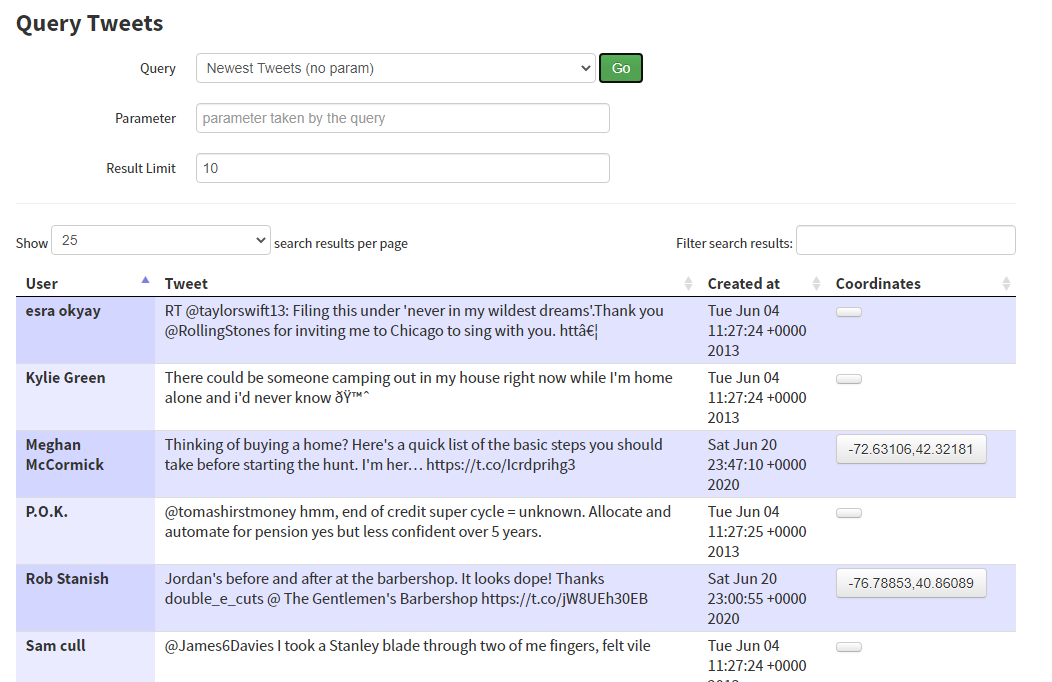
\includegraphics[width=\textwidth,height=\textheight,keepaspectratio]{search_newest_tweets.png}\\
\textbf{getBestMovies}\\
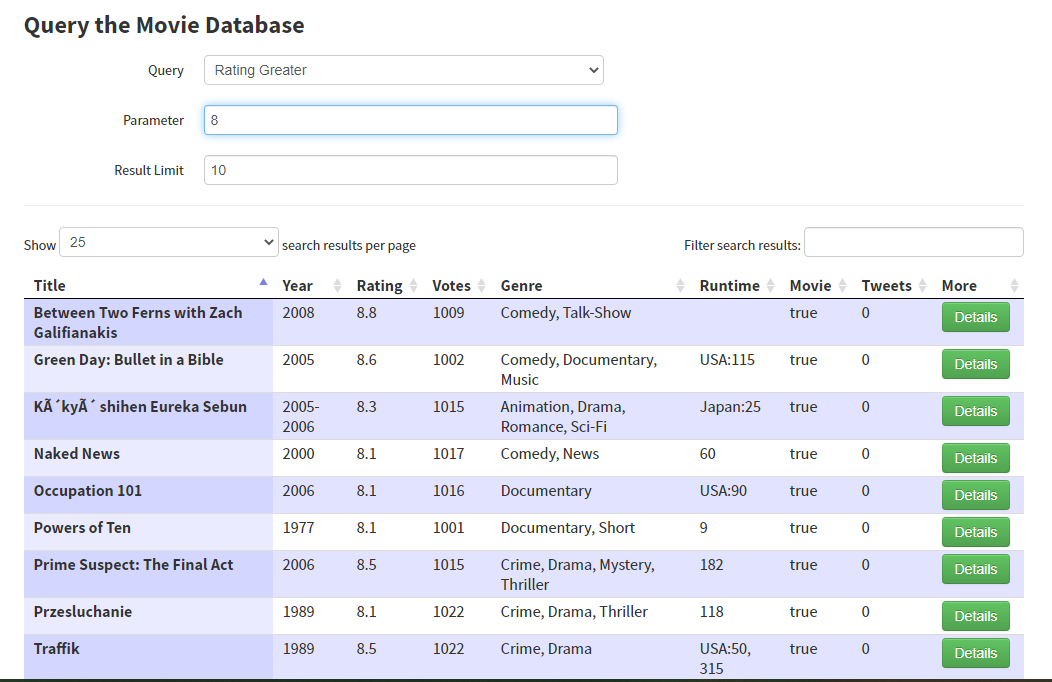
\includegraphics[width=\textwidth,height=\textheight,keepaspectratio]{search_rating.png}\\
\end{document}
